\section{Results}

\begin{figure}[H]
    \centering
    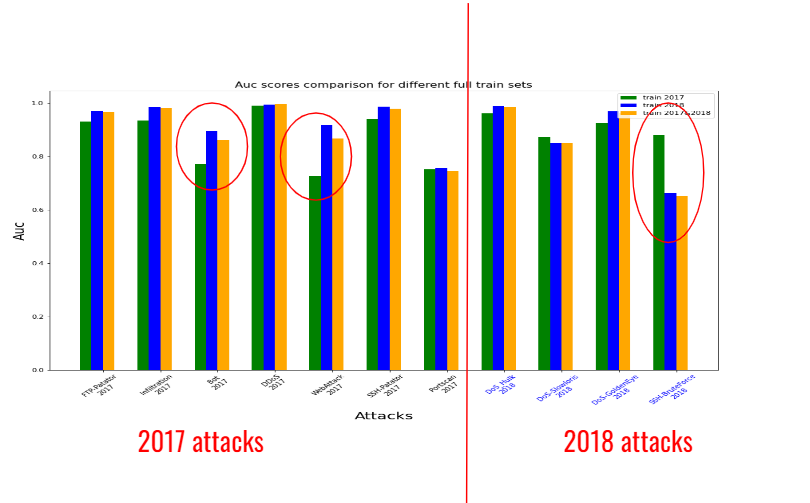
\includegraphics[width=1\linewidth]{augment.png}
    \caption{}
\end{figure}

From our experiments, we can see that using foreign datasets during training increases the AUC score. In Figure 1, when using the 2017 dataset as the test set, training with 2018 dataset or training with both 2017 and 2018 datasets outperforms training with just the 2017 dataset in most attack scenarios. Similarly, when using the 2018 dataset as the test, training with 2017 datasets or combining both datasets outperforms training with just the 2018 dataset. We have highlighted the attacks in which augmenting data with foreign datasets increased performance. As such, we conclude that, in many case, augmenting data benefits the detection system.

\begin{figure}[H]
    \centering
    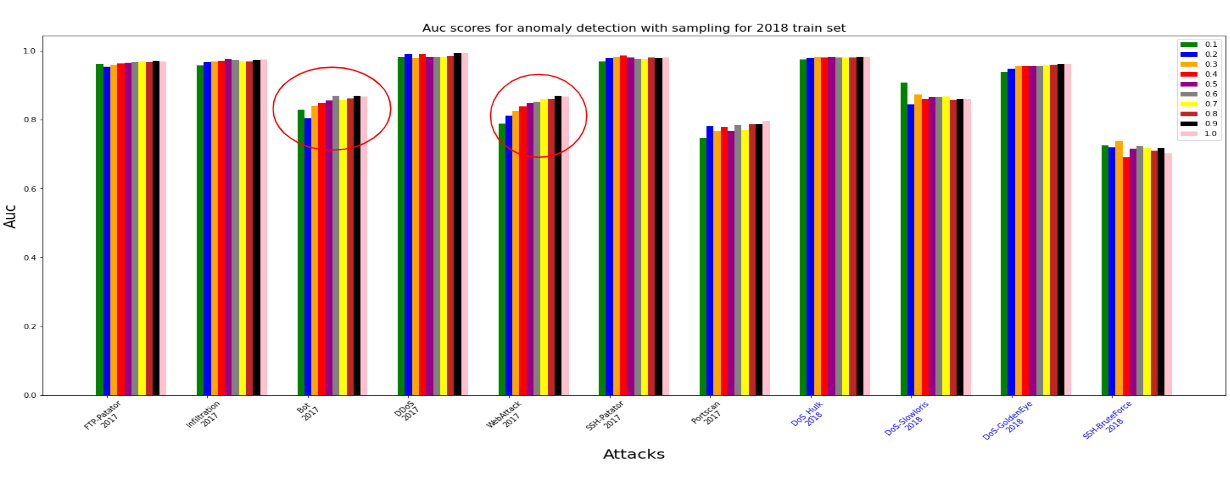
\includegraphics[width=1\linewidth]{amount.png}
    \caption{}
\end{figure}

In Figure 2, we see that only in certain attack scenarios does the amount of the data impact our result. Specifically, the BotNet 2017 and WebAttack 2017 showed strong evidence that increasing the training set size betters the AUC score. In other scenarios, we don't see a strong trend and thus the effect of dataset size on the AUC score is inconclusive.

\begin{figure}[H]
    \centering
    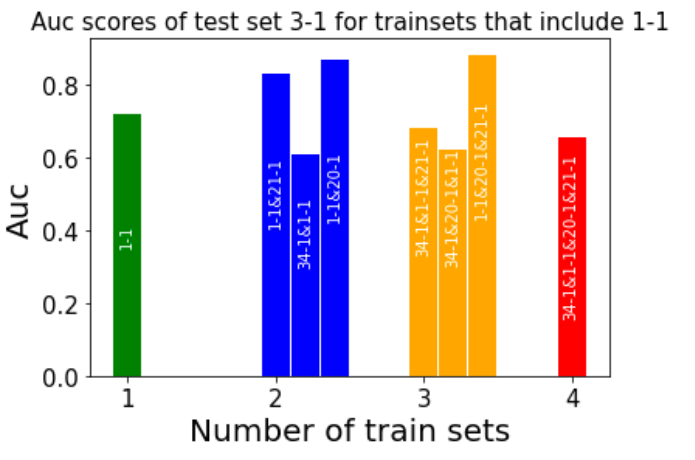
\includegraphics[width=1\linewidth]{data.png}
    \caption{}
\end{figure}

In Figure 3, we augment the data with different, foreign datasets and conclude that there is huge variance in the resulting AUC scores. This means that the type of data shared with the trainer matters as well. However, it's inconclusive exactly what type of data is the most beneficial in different attack scenarios.

\label{sec:results}
